\section{Evaluación del modelo mediante casos hipotéticos}\label{sec:evalmodel-casoshipot}

% Descripción de los tipos de cuarentena y las medidas de cuidado 
Las combinaciones entre los distintos niveles de cuidado y cuarentena presentados en \ref{met:evaluacion-hipot} dan lugar a una serie de casos, los cuales son presentados en la tabla \ref{table:casos-hipoteticos}. Se resuelve el sistema para cada caso, comenzando desde las condiciones iniciales y los parámetros \(\gamma_E, \gamma_I\) estimados con \textit{RTS smoother} en la sección anterior. Se prueban dos escenarios; el primero, en que el \(\beta_{\text{exterior}}\) es un valor mayor pero cercano a \(1\), de tal forma que es la tasa de contagio depende del ambiente hogar, y cuando es un valor mucho más grande que \(1\), de forma que la tasa de contagio está totalmente dominada por el ambiente exterior (todos los contagios ocurren fuera de la casa).


\subsection{Escenario con \(\beta_{\text{exterior}} >> 1\)}

En este caso las infecciones ocurren solamente en el exterior del hogar (las infecciones dentro del hogar son despreciables en comparación). Se utiliza \(\beta_{\text{exterior}} = 68.0\), pero los resultados son similares para un rango amplio de parámetros.


\begin{table}[h!]
\centering
\begin{tabular}{||l| c c c||} 
 \hline
 & \textbf{Cuidado insuficiente} & \begin{tabular}{@{}c@{}}\textbf{Cuidado} \\ \textbf{normal}\end{tabular} & \begin{tabular}{@{}c@{}}\textbf{Cuidado} \\ \textbf{extra}\end{tabular}\\ 
 \hline
 \textbf{Sin cuarentena} & Caso 1 & Caso 2 & Caso 3 \\ 
 \textbf{Cuarentena normal} & Caso 4 & Caso 5 & Caso 6 \\
 \textbf{Cuarentena fuerte} & Caso 7 & Caso 8 & Caso 9 \\
 \hline
\end{tabular}
\caption{Casos hipotéticos para distintas combinaciones de cuarentena y cuidado.}
\label{table:casos-hipoteticos}
\end{table}

Las figuras \ref{img:all-hip-S-N} y \ref{img:all-hip-I-N} presentan la evolución de los susceptibles \(S_i/N_i\) e infectados \(S_i/N_i\) (normalizados por el total de personas en cada clase), para cada uno de los casos. Se utilizan los mismos límites para los ejes \(y\) para facilitar la comparación.

Como era de esperarse, las diferencias socioeconómicas disminuyen debido a que la mayoría de los casos están utilizando, o bien la misma matriz de tiempos de residencia, o bien los mismos factores sanitarios (o ambos).


\begin{table}[h!]
\centering
\begin{tabular}{||m{2.5cm}|m{4cm} m{4cm} m{4cm}||} 
 \hline
 & Cuidado & \begin{tabular}{@{}c@{}}\textbf{Cuidado} \\ \textbf{normal}\end{tabular} & \begin{tabular}{@{}c@{}}\textbf{Cuidado} \\ \textbf{extra}\end{tabular}\\ 
 \hline
 \textbf{Sin cuarentena} & \textit{Caso 1}: Se contagia \(\sim 90\%\) de la población en los primeros 6 meses, de manera uniforme entre las distintas clases. Luego la enfermedad desaparece. & \textit{Caso 2}: Se contagia \(\sim 90\%\) de la población en los primeros 6 meses, de manera uniforme entre las distintas clases. Luego la enfermedad desaparece. & \textit{Caso 3}: Se logra controlar el alza de casos, alcanzando el \textit{peak} de mediados de julio de 2020 y el de inicios de mayo de 2021 con menos de la mitad de casos, e incluso se evita el rebrote de junio de 2021. \\ 
 \textbf{Cuarentena normal} & \textit{Caso 4}: El primer \textit{peak} de julio de 2020 alcanza más del doble de casos y tiene una reducción lenta, de tal forma que el \textit{peak} de mayo de 2021 es apenas registrado como un alza ligera. & \textit{Caso 5}: Desarrollo real de la pandemia, tomado como referencia& \textit{Caso 6}: La enfermedad alcanza un pequeño \textit{peak} en julio de 2020 y luego se extingue.\\
 \textbf{Cuarentena fuerte} & \textit{Caso 7} El primer \textit{peak} es muy similar en fecha y número de infectados, pero con un alza sostenida en el número de casos a partir septiembre de 2020, llegando a un \textit{peak} de más del doble de infectados en julio de 2021. & \textit{Caso 8} Se observan dos \textit{peaks} de unas 5000 personas, similar al Caso 3 pero sin poder contener el rebrote de junio de 2021. & \textit{Caso 9}: La enfermedad se extingue luego de los primeros meses. \\
 \hline
\end{tabular}
\caption{Observaciones para cada caso hipotético, escenario con \(\beta_{\text{exterior}} = 68.\) (el ambiente exterior domina los contagios).}
\label{table:descripcion-casos-hipot}
\end{table}


Se puede ver como en los casos 1 y 2, que corresponden a casos sin cuarentena con cuidado insuficiente o cuidado normal respectivamente, se contagia la gran mayoría de la población dentro de los primeros 6 meses considerados. En el caso con cuidado normal, la clase más acomodada resulta tener una incidencia bastante menor que las demás.

Es interesante que la simulación muestra como el cuidado extra (casos 3, 6 y 9) es suficiente por sí mismo de controlar el alza de casos, incluso sin ningún tipo de cuarentena (caso 3). Con cuarentena (casos 6 y 9), la enfermedad desaparece rápidamente de entre la población en los primeros meses. Esto desde luego no considera importación de casos externos.

% Aquí pongo todos los resultados de casos hipotéticos que obtuve... cuarentenas fuertes, etc... 
% \begin{figure}[h]
% \centering
% \includegraphics[width=0.99\textwidth]{img/resultados/allhipcases_S-N_commonylim0_1\parameterstring}
% \caption{Estimación de susceptibles, normalizados por el total de cada grupo \(S_i/N_i\), para cada caso hipotético.}
% \label{img:all-hip-S-N}
% \end{figure}

% \begin{figure}[h]
% \centering
% \includegraphics[width=0.99\textwidth]{img/resultados/allhipcases_I-N_commonylim0-015\parameterstring}
% \caption{Estimación de infectados normalizados por el total de cada grupo \(I_i/N_i\), para cada caso hipotético.}
% \label{img:all-hip-I-N}
% \end{figure}

La figura \ref{img:hip-3478-I-comp} muestra cuatro casos interesantes, comparándolos con la situación normal. 




En estos tres casos, el impacto es mayor sobre la clase 5 (la más vulnerable). Esto puede atribuirse al hecho de que es esa la clase que presenta en general un mayor factor sanitario y movilidad.
 
 

% Fechas 
% important_dates = [
%    Date(2020, 5, 13), # cuarentena total en la RM
%    Date(2020, 10, 25), # plesbicito por nueva constitución
%    Date(2021, 1, 4), # comienza a regir el permiso de vacaciones
%    Date(2021, 2, 1), # comienza un plan de vacunación más fuerte (según datos)
%    Date(2021, 5, 26) # un 50% de la población de Santiago tiene la primera dosis
%]
% casos interesantes: 3, 4, 7, 8

\begin{figure}
     \centering
     \begin{subfigure}[b]{.47\textwidth}
         \centering
         \includegraphics[width=\textwidth]{img/resultados/comparecase_3withnormal_I_\parameterstring}
         \caption{Caso \(3\): Cuidado extra sin cuarentena.}
     \end{subfigure}
     \hfill
     \begin{subfigure}[b]{.47\textwidth}
         \centering
         \includegraphics[width=\textwidth]{img/resultados/comparecase_4withnormal_I_\parameterstring}
         \caption{Caso \(4\): Cuidado insuficiente y cuarentena normal.}
     \end{subfigure}
     \hfill
     \begin{subfigure}[b]{.47\textwidth}
         \centering
         \includegraphics[width=\textwidth]{img/resultados/comparecase_7withnormal_I_\parameterstring}
         \caption{Caso \(7\): Cuidado insuficiente y cuarentena fuerte.}
     \end{subfigure}
     \hfill
     \begin{subfigure}[b]{.47\textwidth}
         \centering
         \includegraphics[width=\textwidth]{img/resultados/comparecase_8withnormal_I_\parameterstring}
         \caption{Caso \(8\): Cuidado normal y cuarentena fuerte.}
     \end{subfigure}
        \caption[Personas infectadas para caso hipotéticos seleccionados.]{Personas infectadas para caso hipotéticos seleccionados, con la estimación de los casos reales de fondo. Diferentes límites para el eje \(y\). Las líneas grises corresponden a las fechas relevantes de la tabla \ref{table:fechas-relevantes}.}
        \label{img:hip-3478-I-comp}
\end{figure}


\subsection{Escenario con \(\beta_{\text{exterior}} \approx 1\)}

En este caso se buscó un valor donde existiera contagio en el hogar, y se eligió \(\beta_{\text{exterior}} = 1.2\). Se observa que la cuarentena prácticamente no influye en el número de contagios; lo que realmente determina si se controla o no la pandemia es el factor sanitario. Los resultados se sintetizan en la tabla \ref{table:descripcion-casos-hipot-beta-1-2}, y los casos de interés elegidos anteriormente se presentan en la figura \ref{img:hip-3478-I-comp-beta1-2}.



\begin{table}[h!]
\centering
\begin{tabular}{||m{2.5cm}|m{4cm} m{4cm} m{4cm}||} 
 \hline
 & Cuidado & \begin{tabular}{@{}c@{}}\textbf{Cuidado} \\ \textbf{normal}\end{tabular} & \begin{tabular}{@{}c@{}}\textbf{Cuidado} \\ \textbf{extra}\end{tabular}\\ 
 \hline
 \textbf{Con o sin cuarentena} & \textit{Casos 1, 4 y 7}: Se observan \textit{peaks} de más del doble de casos que el normal, y que se reducen más lentamente. El número de contagios no baja del \(0.5\%\) de la población.  & \textit{Caso 2, 5 y 8} Muy similares al caso 5, el normal usado como referencia. & \textit{Caso 3, 6, y 9}: La enfermedad tiene un pequeño \textit{peak} en torno a julio de 2020 y se extingue luego de unos meses. \\
 \hline
\end{tabular}
\caption[Observaciones para cada caso hipotético, escenario con \(\beta_{\text{exterior}} = 1.2\)]{Observaciones para cada caso hipotético, escenario con \(\beta_{\text{exterior}} = 1.2\) (el ambiente hogar también juega un rol en el contagio). Se condensan la tabla, puesto que no hay variaciones importantes con respecto a la fuerza de la cuarentena.}
\label{table:descripcion-casos-hipot-beta-1-2}
\end{table}



\begin{figure}
     \centering
     \begin{subfigure}[b]{.47\textwidth}
         \centering
         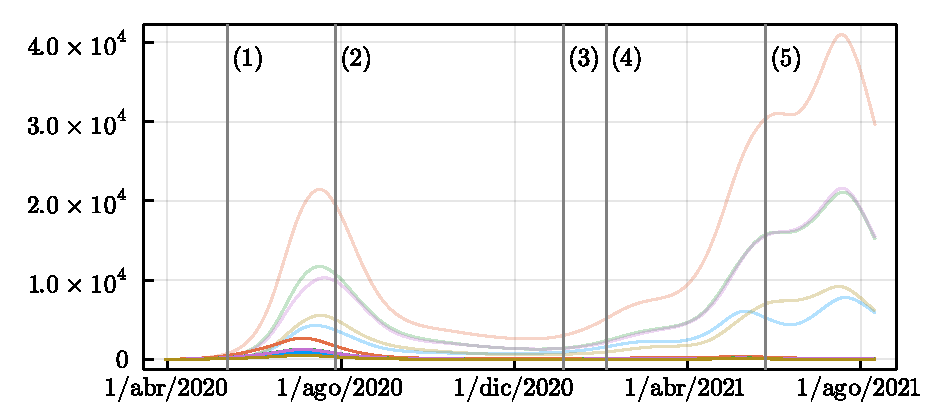
\includegraphics[width=\textwidth]{img/resultados/comparecase_3withnormal_I_gamma_e_0-1724_gamma_i_0-0833_beta_2_2-0000.pdf}
         \caption{Caso \(3\): Cuidado extra sin cuarentena.}
     \end{subfigure}
     \hfill
     \begin{subfigure}[b]{.47\textwidth}
         \centering
         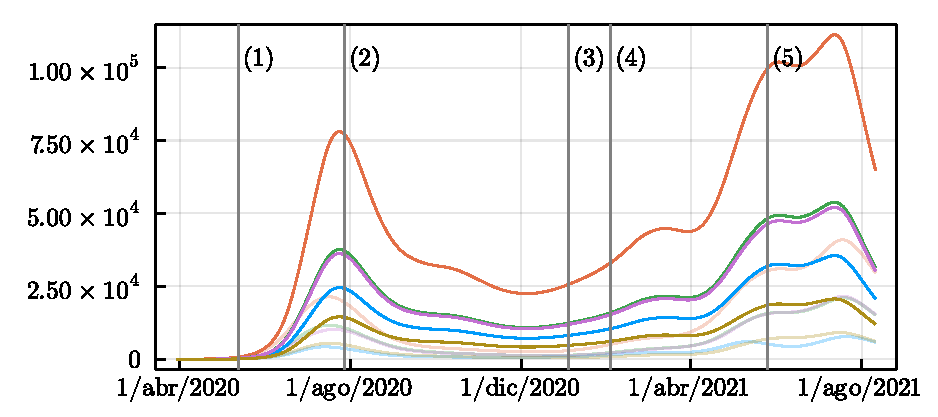
\includegraphics[width=\textwidth]{img/resultados/comparecase_4withnormal_I_gamma_e_0-1724_gamma_i_0-0833_beta_2_2-0000.pdf}
         \caption{Caso \(4\): Cuidado insuficiente y cuarentena normal.}
     \end{subfigure}
     \hfill
     \begin{subfigure}[b]{.47\textwidth}
         \centering
         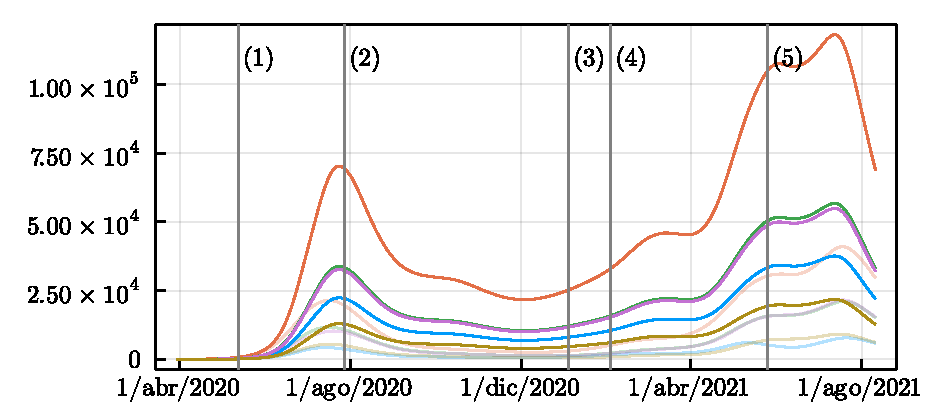
\includegraphics[width=\textwidth]{img/resultados/comparecase_7withnormal_I_gamma_e_0-1724_gamma_i_0-0833_beta_2_2-0000.pdf}
         \caption{Caso \(7\): Cuidado insuficiente y cuarentena fuerte.}
     \end{subfigure}
     \hfill
     \begin{subfigure}[b]{.47\textwidth}
         \centering
         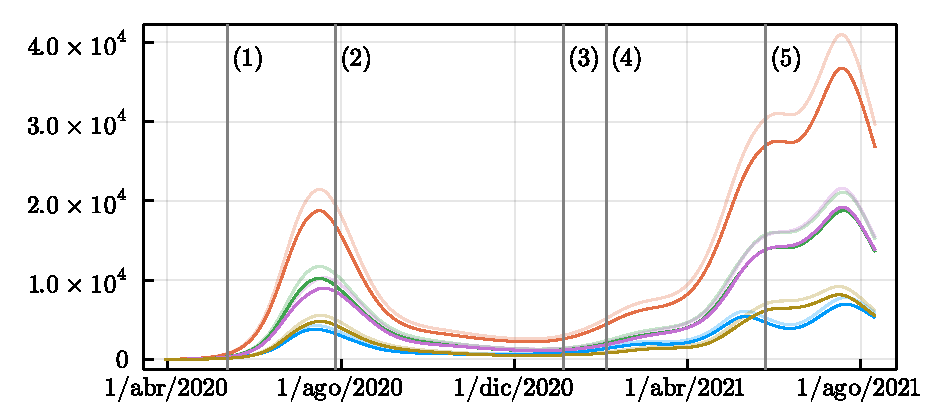
\includegraphics[width=\textwidth]{img/resultados/comparecase_8withnormal_I_gamma_e_0-1724_gamma_i_0-0833_beta_2_2-0000.pdf}
         \caption{Caso \(8\): Cuidado normal y cuarentena fuerte.}
     \end{subfigure}
        \caption[Personas infectadas para caso hipotéticos seleccionados.]{Personas infectadas para caso hipotéticos seleccionados, con la estimación de los casos reales de fondo. Diferentes límites para el eje \(y\). Las líneas grises corresponden a las fechas relevantes de la tabla \ref{table:fechas-relevantes}.}
        \label{img:hip-3478-I-comp-beta1-2}
\end{figure}
